%!TEX root = thesis.tex

\chapter{John von Neumann}
\section{Herkunft und Anfänge seiner Karriere}

\begin{figure}[ht]
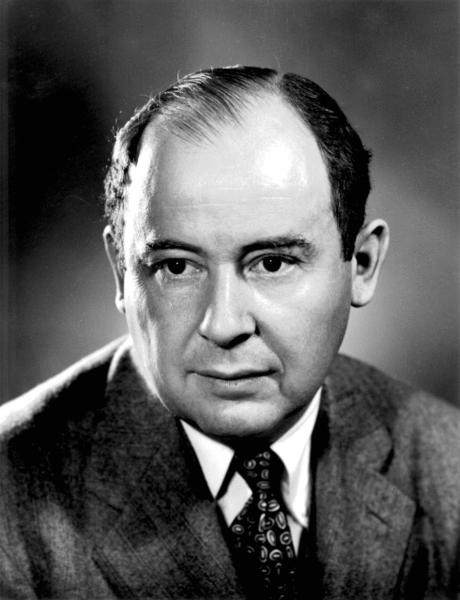
\includegraphics[width=0.3\textwidth]{jvn.png}
\caption{John von Neumann, 1940}
\end{figure}
János Neumann entstammte einer jüdischen Bankiersfamilie. Sein Vater, der königlich ungarische Regierungsrat Max Neumann, wurde am 1. Juli 1913 in den ungarischen Adelsstand erhoben. Schon als Kind zeigte John Neumann jene überdurchschnittliche Intelligenz, die später selbst Nobelpreisträger – zum Beispiel Eugene Paul Wigner – zum Staunen brachte. Als Sechsjähriger konnte er mit hoher Geschwindigkeit achtstellige Zahlen im Kopf dividieren. Er besaß ein außergewöhnliches Gedächtnis, das ihm beispielsweise erlaubte, den Inhalt einer Buchseite nach einem kurzen Blick darauf präzise wiederzugeben. Später konnte er ganze Bücher wie Goethes Faust auswendig und so zum Beispiel auch durch detailliertes historisches Wissen glänzen. Er besuchte in Budapest das humanistische deutschsprachige Lutheraner-Gymnasium, wie auch gleichzeitig Eugene Paul Wigner. Schon als Gymnasiast glänzte er durch mathematische Leistungen und veröffentlichte mit 17 Jahren seinen ersten mathematischen Artikel. Dem Wunsch seiner Eltern folgend, studierte er jedoch zunächst von 1921 bis 1923 Chemieingenieurwesen in Berlin und dann bis zu seinem Diplom an der ETH Zürich. Sein eigentliches Interesse galt allerdings immer der Mathematik, der er sich gewissermaßen als „Hobby“ widmete. Er besuchte, da er in Budapest zunächst nicht zugelassen wurde (Kontingentierung für Juden), Mathematikkurse von Hermann Weyl und George Pólya an der ETH und machte schon bald auf sich aufmerksam. Von Neumann war von 1928 bis 1933 (jüngster) Privatdozent der Berliner Universität und im Sommersemester 1929 an der Universität Hamburg. Davor arbeitete er 1926/1927 in Göttingen mit David Hilbert zusammen.

Am Anfang seiner Karriere als Mathematiker beschäftigte sich von Neumann unter anderem mit der Entwicklung der axiomatischen Mengenlehre, für die er noch als Student einen neuen Ansatz fand (Dissertation in Budapest 1926 bei Leopold Fejér), und mit der Hilbertschen Beweistheorie. Diese Themen waren damals das aktuelle Forschungsgebiet der Gruppe um Hilbert in Göttingen, damals noch eines der Weltzentren der Mathematik. Seine Definition der Ordinalzahlen ist heute ein Standard: Eine neue Ordinalzahl wird durch die Menge der bereits eingeführten definiert. Die Phase seiner Beschäftigung mit mathematischer Logik endete mit dem Bekanntwerden von Gödels Unvollständigkeitssatz, der Hilberts Programm einen schweren Schlag versetzte. Gödel war später ein enger Freund und Kollege von Neumann und Albert Einstein in Princeton.

\section{Arbeiten zur Quantenmechanik}

Von Neumann war ebenfalls Verfasser des ersten mathematisch durchdachten Buches zur Quantenmechanik, in dem er den Messprozess und die Thermodynamik der Quantenmechanik behandelte (siehe dazu Dichtematrix, von ihm 1927 eingeführt, von-Neumann-Entropie). Das damals „heiße“ Thema der sich stürmisch entwickelnden Quantenmechanik war auch der Hauptgrund, warum er sich der Funktionalanalysis zuwandte und die Theorie linearer Operatoren in Hilberträumen entwickelte, genauer die der unbeschränkten selbstadjungierten Operatoren. Die Mathematiker in Göttingen wandten gegen die neue Quantenmechanik ein, dass mit den bis dahin untersuchten linearen beschränkten Operatoren die kanonischen Vertauschungsrelationen nicht zu erfüllen waren. Von Neumann klärte das und lieferte gleichzeitig zahlreiche weitere Beiträge zu diesem Gebiet. Als man allerdings später Werner Heisenberg fragte, ob er von Neumann deswegen nicht dankbar sei, stellte er nur die Gegenfrage, wo denn der Unterschied zwischen beschränkt und unbeschränkt liege.\cite{bams} Von Neumanns Buch über Quantenmechanik genoss einen derartigen Ruf, dass selbst sein „Beweis“ der Unmöglichkeit von Hidden-Variable-Theorien, der zwar korrekt war, aber von falschen Voraussetzungen ausging, lange nicht hinterfragt wurde. Die Physiker bevorzugten jedoch zu von Neumanns Leidwesen die fast gleichzeitig veröffentlichten Principles of Quantum mechanics von Paul Dirac, in der das angesprochene mathematische Problem durch Einführung von Distributionen umgangen wurde, die bei den Mathematikern zunächst verpönt waren, ehe sie auch dort Ende der 1940er Jahre ihren Siegeszug antraten (Laurent Schwartz).

Mit Eugene Wigner veröffentlichte von Neumann 1928/29 eine Reihe von Arbeiten über die Anwendung der Gruppentheorie in den Atomspektren. Auch hier war die Begeisterung der Physiker gedämpft, es wurde sogar von „Gruppenpest“ gesprochen, die sich von Seiten der Mathematiker in der Quantenmechanik breitzumachen versuchte.

Das Stone-von Neumann-Theorem drückt die Eindeutigkeit der kanonischen Kommutatoren von zum Beispiel Orts- und Impulsoperatoren in der Quantenmechanik aus und zeigt die Äquivalenz von deren beiden grundlegenden Formulierungen von Schrödinger (Wellenfunktion) und Heisenberg (Matrizen).

Seine Arbeiten über Quantenmechanik begründeten seinen Ruf in Amerika – und nicht zuletzt im Hinblick auf einen Wechsel auf besser bezahlte Positionen in den USA hat er sich so intensiv mit ihr beschäftigt. Im Herbst 1929 wurde er von Oswald Veblen eingeladen, an die Princeton University in New Jersey zu kommen und Vorträge darüber zu halten, und er wechselte auch in den folgenden Jahren zwischen Princeton und Deutschland. Ab 1933 wirkte er am neu gegründeten, anspruchsvollen Institute for Advanced Study in Princeton als Professor für Mathematik. Einige seiner Kollegen dort waren Albert Einstein und Hermann Weyl. Wie diese emigrierte auch von Neumann nach der Machtergreifung Hitlers dauerhaft in die USA.

\section{Amerika, Spieltheorie und anderes}

John von Neumann erbrachte auf vielen Gebieten der Mathematik herausragende Beiträge. Schon 1928 hatte ihn ein Aufsatz des Mathematikers Émile Borel über Minimax-Eigenschaften zu Ideen geführt, die später auf einen seiner originellsten Entwürfe hinausliefen, die Spieltheorie. Von Neumann bewies 1928 das Min-Max-Theorem für die Existenz einer optimalen Strategie in „Nullsummenspielen“. Mit dem Wirtschaftswissenschaftler Oskar Morgenstern schrieb er 1944 das zum Klassiker gewordene Buch The Theory of Games and Economic Behavior (3. Auflage 1953), wo auch die für die Ökonomie wichtige Verallgemeinerung auf n-Personen Spiele behandelt wird. Er wurde damit zum Begründer der Spieltheorie, die er allerdings weniger auf klassische Spiele anwendet, als auf alltägliche Konflikt- und Entscheidungssituationen bei unvollkommener Kenntnis der Absichten des Gegenspielers (wie beim Pokern). In den Wirtschaftswissenschaften wird auch ein Seminarvortrag von 1936 zur mathematischen Modellierung expandierender Wirtschaften häufig zitiert. In der zweiten Auflage von The Theory of Games and Economic Behavior (1947) präsentierten Morgenstern und von Neumann den Von-Neumann-Morgenstern-Erwartungsnutzen und leisteten damit bedeutende Beiträge zur Nutzentheorie.

In den 1930er Jahren entwickelte von Neumann\cite{games} in einer Serie von Arbeiten mit Francis Murray eine Theorie von Algebren beschränkter Operatoren in Hilberträumen, die Jacques Dixmier später von-Neumann-Algebren nannte. Diese sind heute ein aktuelles Forschungsgebiet (zum Beispiel Alain Connes, Vaughan F. R. Jones), das auch – wie von Neumann vorhersah – Anwendungen in der Physik hat, allerdings weniger in der Quantenmechanik als in der Quantenfeldtheorie und Quantenstatistik. Von Neumann und Murray bewiesen ein Klassifikationstheorem für Operatoralgebren als direkte Summe von „Faktoren“ (mit trivialem Zentrum) vom Typ I, II, III, jeweils mit Unterteilungen.

Operatoralgebren waren Teil seiner Suche nach einer Verallgemeinerung des quantenmechanischen Formalismus, denn er sagte in einem Brief an Birkhoff 1935, er würde nicht mehr an Hilberträume glauben. Weitere Versuche in dieser Richtung waren die Untersuchung der „lattice theory“ (Theorie der Verbände), zunächst als Algebra von Projektionsoperatoren im Hilbertraum (an der auch Birkhoff beteiligt war), später als Erweiterung der Logik zur „Quantenlogik“ interpretiert, und kontinuierliche Geometrien, die sich aber am Ende als kein Fortschritt gegenüber Operatoralgebren erwiesen.

Ein weiteres Arbeitsfeld der 1930er Jahre in Princeton war das berühmte Ergodenproblem, bei dem es um die mathematische Grundlegung der statistischen Mechanik in klassischen Systemen geht (Gleichverteilung der Bahnen im Phasenraum). Von Neumann hatte in Deutschland diese Fragen schon von quantenmechanischer Seite behandelt. Nachdem Bernard Koopman das Problem in Operator-Form gebracht hatte, griff von Neumann es auf und lieferte sich unfreiwillig ein „Duell“ mit dem bekannten amerikanischen Mathematiker George David Birkhoff. Wie er später sagte, hätte er eine Zusammenarbeit vorgezogen.

Von Neumann war einerseits geschätzt, weil er seine Ideen freigiebig weitergab und Kollegen weiterhalf (bei Besuchen in Los Alamos war er oft von einer Traube von Wissenschaftlern umgeben, die schnellen Rat wollten), andererseits gefürchtet, da er Ideen schnell aufgriff und mit atemberaubender Geschwindigkeit eigene Theorien daraus entwickelte.

\section{Manhattan-Projekt und Regierungsberater}

Von Neumann arbeitete ab 1943 am Manhattan-Projekt in Los Alamos. Er war schon in den Jahren zuvor bei der Army und Navy ein gefragter Berater (Ballistikfragen aller Art, Hohlladungen, operations research, Bekämpfung deutscher Magnetminen, Optimierung der Wirkung von Bomben mit „schrägen Stoßwellen“ usw.). Eines seiner Hauptarbeitsgebiete war denn auch die Theorie der Stoßwellen, die in den 50er Jahren für den Überschallflug aktuell wurde und die er unter anderem für die Entwicklung von Sprengstofflinsen für den Implosionsmechanismus der Plutoniumbombe nutzte. In diesen Zusammenhang gehört auch seine Entwicklung des ersten numerischen Verfahrens zur Lösung von hyperbolischen partiellen Differentialgleichungen, des Monte-Carlo-Verfahrens mit Stanislaw Ulam, die von-Neumann-Stabilitätsanalyse sowie seine Pionierleistungen in der Rechnerarchitektur. Übrigens optimierte er mit seiner Expertise in der Theorie der Stoßwellen während des Zweiten Weltkriegs auch englische Luftminen über Deutschland. Auch an der Weiterentwicklung des amerikanischen Nuklearbomben-Programms bis hin zur Wasserstoffbombe war von Neumann beteiligt.

Neben seinen mathematischen Leistungen war von Neumann als Regierungsberater auch politisch einflussreich. Vor dem Abwurf der Atombomben auf Japan war er ein Mitglied des Target Committee, das die genauen Ziele der Bomben mitbestimmte. Er berechnete dabei auch die optimale Detonationshöhe der Atombomben, um einen möglichst großen Schaden durch die Explosion am Boden zu erzielen. Mit dem Namen John von Neumann ist angeblich auch die Idee verbunden, die Ost-West-Konfrontation durch die Explosion einer Wasserstoffbombe über unbewohntem sowjetischem Gebiet zu beenden, die Sowjetunion von der Entwicklung einer eigenen Bombe abzuhalten und dauerhaft einzuschüchtern. Ob US-Präsident Eisenhower allerdings tatsächlich durch von Neumann zu einem solchen Schritt gedrängt wurde, ist umstritten. Er war aber wesentlich daran beteiligt, das militärische Raketenprogramm der USA auf den Weg zu bringen.

\section{Arbeiten zum Computer}

\begin{figure}[ht]
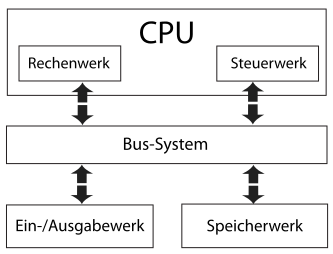
\includegraphics[width=0.3\textwidth]{vna.png}
\caption{Veranschaulichung der Von-Neumann-Architektur}
\end{figure}
Von Neumann gilt als einer der Väter der Informatik. Nach ihm wurde die Von-Neumann-Architektur (auch Von-Neumann-Rechner) benannt, ein Computer, in dem Daten und Programm binär codiert im selben Speicher liegen. Das Programm selbst kann somit im laufenden Rechenvorgang verändert werden und durch bedingte Sprungbefehle von der festgelegten Reihenfolge der gespeicherten Anweisungen abgewichen werden. Es definiert in loser Analogie zum menschlichen Hirn (wie er im Report schreibt) eine Rechnerarchitektur aus Steuereinheit und arithmetischer Einheit sowie eine Speichereinheit. Die Befehle werden seriell abgearbeitet. Er beschrieb dieses Prinzip 1945 im First Draft of a Report on the EDVAC. Der Bericht war als Diskussionsbericht mit der ENIAC-Gruppe gedacht und blieb zunächst unveröffentlicht, kursierte jedoch schnell in wissenschaftlichen Kreisen. So gut wie alle modernen Rechner beruhen auf von Neumanns Idee.

Von Neumanns Rolle als alleiniger Erfinder der nach ihm benannten modernen Rechnerarchitektur ist bestritten worden und seit längerem Gegenstand von Auseinandersetzungen. Heutzutage wird deshalb vorzugsweise statt „Von-Neumann-Rechner“ die Bezeichnung „speicherprogrammierter Rechner“ (stored program computer) verwendet. Insbesondere betrifft das die Ansprüche der eigentlichen Erbauer des ersten Röhrencomputers ENIAC und dessen Nachfolgemodells EDVAC, John Presper Eckert und John William Mauchly von der Moore School der University of Pennsylvania in Philadelphia, mit denen von Neumann und Herman Goldstine anfangs eng zusammenarbeiteten. Von Neumann stieß durch eine zufällige Begegnung auf einem Bahnsteig mit dem ihm zuvor nicht bekannten Mathematiker Goldstine im August 1944 zu den Computerentwicklern der Moore School, wo Goldstine Verbindungsoffizier der US-Army war. Wie Goldstine berichtete, beendete die von ihm selbst betriebene freizügige Verbreitung des Edvac-Reports die enge Beziehung von ihm und von Neumann zu Eckert und Mauchly, die ihren Beitrag in dem (eigentlich nicht für die Öffentlichkeit bestimmten) Edvac-Report nicht gewürdigt sahen und für wesentliche Teile des Von-Neumann-Rechners Prioritätsansprüche geltend machten. Bei Eckert und Mauchly standen Patentüberlegungen im Vordergrund, die dazu führten, dass sie schon 1946 die Moore School verließen, um eine eigene Firma zu gründen, und die später zu einem jahrzehntelangen Streit vor Gericht führten (sie schalteten schon 1945 Patentanwälte ein). Von Neumann sah dagegen zunächst Bedarf für weitere Forschung und Entwicklung und trat für eine offene Diskussion und weite Verbreitung der Ergebnisse ein. Teile des Konzepts wurden unabhängig auch von anderen Computerpionieren – darunter Konrad Zuse in Deutschland – entwickelt, u. a. die Idee der Trennung von Speicher und Prozessor, die schon in Zuses noch rein mechanischen Z1 im Jahr 1938 erfolgte. Zuses frühen Rechnern, die für Spezialaufgaben ausgelegt waren, fehlte jedoch das wesentliche Konzept der bedingten Verzweigung, obwohl es ihm bekannt war und er es in seinem Plankalkül verwendete. Von Neumann setzte sich seinerzeit vehement für die weitere Entwicklung der Rechenmaschinen ein. Die Verdienste von Neumanns beruhen insbesondere auf der Mathematisierung und Verwissenschaftlichung der Rechenmaschinen.\cite{vna}

Von Neumann leitete ab 1949 am Institute for Advanced Study schließlich ein eigenes Computerprojekt, den IAS-Computer, in dem er seine Ideen verwirklichen konnte, darunter auch viele Programmierkonzepte. Auf ihn gehen Unterprogramme mit Parameterübergabe über einen Verweis auf eine Speicherstelle, verschiedene Verfahren zur Erzeugung von Zufallszahlen (unter anderem die Mittquadratmethode und die Verwerfungsmethode) und der Mergesort zurück. Er trug maßgeblich zur Verwendung von Binärcodes in den Rechnersystemen bei und propagierte die Verwendung von Flussdiagrammen, in denen er auch eine Art von Assertions vorsah, die als Vorläufer für Schleifeninvarianten im Hoare-Kalkül angesehen werden können. Ein enger Mitarbeiter wurde Goldstine, den er aus der ENIAC-Gruppe übernahm. Auch die Reports aus Princeton ab 1949 ließ er frei zirkulieren, und schon bald entstanden überall in den USA und England Rechner nach diesen Vorbildern. Genutzt wurde der IAS-Rechner und der nach von Neumanns Ideen umgebaute ENIAC vor allem für militärische Berechnungen (Ballistik). Von Neumann nutzte den Princeton-Rechner allerdings auch für Pionierarbeiten in der numerischen Wettervorhersage, wie die erste rechnergestützte 24-Stunden-Wetterprognose.

1953 entwickelte er auch die Theorie selbstreproduzierender Automaten (von Burks 1966 als Theory of self reproducing automata herausgegeben), für die er ein kompliziertes Beispiel angab (heute ergeben sich viel einfachere aus der Theorie der zellulären Automaten, zum Beispiel John Horton Conways Spiel des Lebens). Ideen dafür soll er auch beim Spielen mit einem Bauklötzchen-Spiel (Tinkertoy) ausprobiert haben. Science-Fiction-Autoren stellten sich die Besiedlung unserer Galaxie mit solchen Automaten vor und prägten dafür den Namen Von-Neumann-Sonden.

\section{Würdigung und Ende}

Über von Neumann kursierten zahlreiche Anekdoten (einige hat Halmos in dem in der Literatur zitierten Artikel gesammelt). Beispielsweise versuchte jemand ihn durch folgendes Rätsel zu testen: „Die Endpunkte einer Strecke s bewegen sich mit der Geschwindigkeit v aufeinander zu, ein Läufer flitzt zwischen den beiden Endpunkten mit einer Geschwindigkeit w > v hin und her. Welche Strecke legt er zurück?“ Es gibt eine einfache und eine etwas kompliziertere Lösungsmethode (Summation der Teilstrecken). Von Neumann gab die Antwort blitzschnell und erklärte auf Nachfrage, die Reihe summiert zu haben – er hatte also den komplizierten Weg gewählt, was für ihn jedoch keinen höheren Zeitaufwand bedeutete.

Wegen seiner Fähigkeit, komplexe Sachverhalte schnell in einfache Fragestellungen zu zergliedern und oft aus dem Stand einer Lösung zuzuführen, sowie seiner streng sachbezogenen, jeden unnötigen Streit vermeidenden Haltung wurde von Neumann gerne als technischer Berater engagiert (so von IBM, Standard Oil, RAND Corporation u. a.), sodass sein Name in zahlreichen Anwendungsgebieten ein Begriff ist. Beispielsweise veröffentlichte er 1952 das Von-Neumann-Gesetz, das die zeitliche Änderung der Größe von Zellen zweidimensionalen Schaumes beschreibt. Für Standard Oil half er Methoden zu entwickeln, Öl-Lagerstätten besser auszunutzen. Sein Tod verhinderte eine geplante größere Zusammenarbeit mit IBM. Für die RAND Corporation wandte er die Spieltheorie auf strategische Denkspiele an, wie auch gleichzeitig andere Mathematiker wie John Nash und John Milnor. In einer unveröffentlichten Arbeit 1953 legte er auch die Prinzipien des Halbleiterlasers dar.

John von Neumann war ein lebenslustiger und geselliger Mensch (Spitzname „Good Time Johnny“); er war zweimal verheiratet (Marietta Kövesi und Klára Dán) und hatte eine Tochter (Marina). Sein Haus in Princeton war Mittelpunkt der akademischen Kreise auf den legendären Princeton-Partys. Von Neumann liebte auch schnelle Wagen (Cadillac, Studebaker), sein Fahrstil war aber gefürchtet, da er sich bei ruhigem Verkehr schnell langweilte und dann in Geistesabwesenheit verfiel. Auch mitten aus einer Party konnte er sich plötzlich verabschieden, um ein mathematisches Problem zu durchdenken. Sein Alkoholkonsum war teilweise nur vorgetäuscht, wie das Kind eines Gastes einmal überrascht feststellte. Ein weiterer Aspekt des „Unterhaltungskünstlers“ von Neumann war sein unerschöpfliches Reservoir oft schlüpfriger Witze und seine Vorliebe für Limericks.

Von Neumann starb nach einem qualvollen Krebsleiden, das möglicherweise durch seine Teilnahme an Nukleartests verursacht worden war, im Washingtoner Walter-Reed-Militärkrankenhaus. Ein Soldat hielt vor dem Zimmer Wache, damit er im Delirium (der Krebs griff am Ende auch sein Gehirn an) keine Staatsgeheimnisse weitergab. Noch auf dem Totenbett schrieb er an seinem Buch „Die Rechenmaschine und das Gehirn“, in dem er den Besonderheiten des „Computers“ im menschlichen Kopf nachging. Er gilt als einer der genialsten und vielseitigsten Mathematiker des 20. Jahrhunderts.